
\section{Mobile App}

    \subsection{Overview}
The mobile app is used to visualize 3D models, access files from the website, and scan QR codes. It is an Android application using ARCore, Google's newest augmented reality library.
    \subsection{Technologies Used}
The Android app is developed in Android Studio, primarily with the Java programming language. The following libraries were used in this project:
    \begin{itemize}
        \item ARCore - Support for AR on Android devices (off of the Google Play Store)
        \begin{itemize}
            \item Only works on specific devices (as of 4/26/2018)
            \item Use OpenGL to draw models, ARCore only performs tracking/world mapping
        \end{itemize}
        \item Obj Parser
        \begin{itemize}
            \item Used by the example AR Core application to draw the model
            \item Parses the obj files
            % \item \url{https://github.com/JohnLXiang/arcore-sandbox}
        \end{itemize}
        \item QR Code Reader - Included in Android project dependencies
        \item Volley - Google library for network communications between app and website
        \item Room - Google library that provides an abstraction layer over SQLite for storing file listings in the phone's database.
    \end{itemize}

    \subsection{Design Details}
    
    \subsubsection{Overview}
        
        The mobile app software is written in Android Studio in the Java programming language. It is an object oriented program with "activities" being the different screens that users can move between. The app has four main screens which are the login, file listing, QR code reader, and AR viewer.
        
        \begin{figure}[H]
            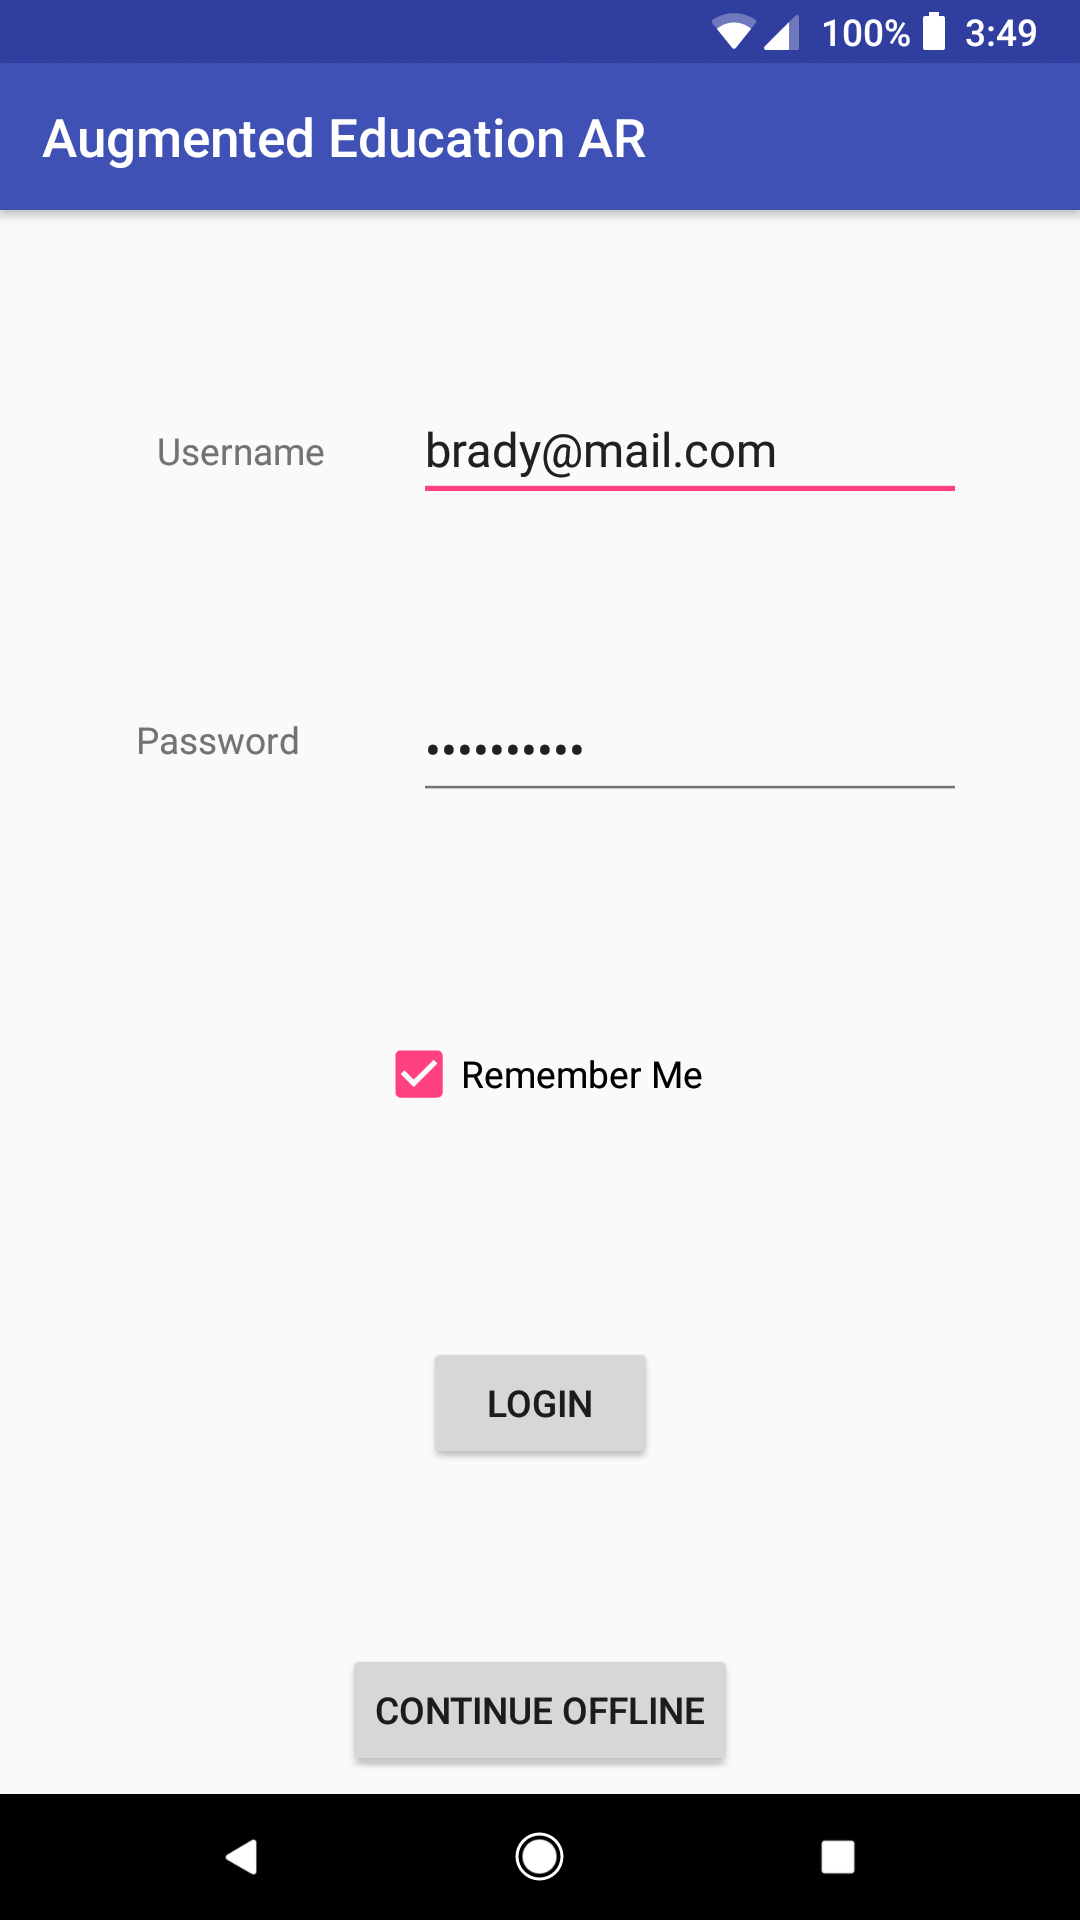
\includegraphics[width=0.5\textwidth]{Mobile/Mobile_MainActivity}
            \centering
            \caption{Mobile App - Login}
            \label{fig:mobileLoginActivity}
        \end{figure}

        \begin{figure}[H]
            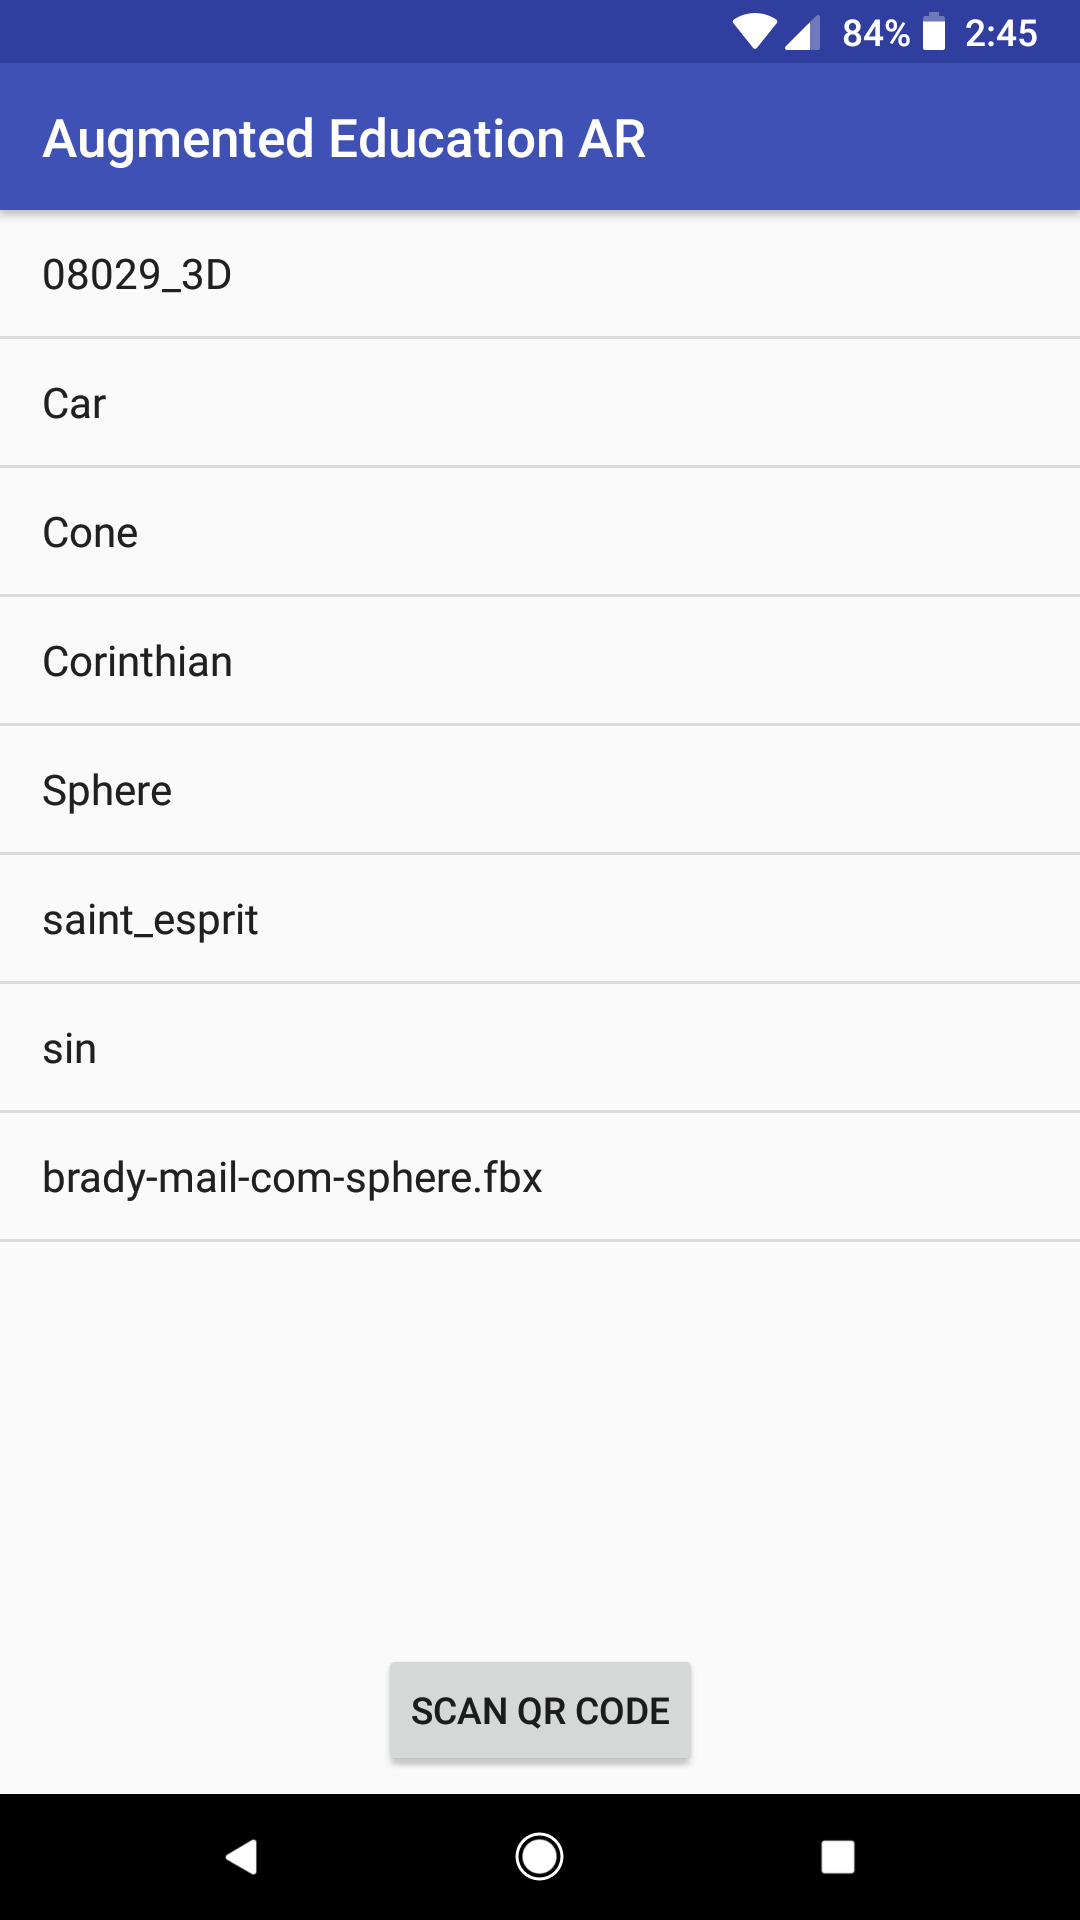
\includegraphics[width=0.5\textwidth]{Mobile/Mobile_ModelList}
            \centering
            \caption{Mobile App - Model Listing}
            \label{fig:mobileModelList}
        \end{figure}

        \begin{figure}[H]
            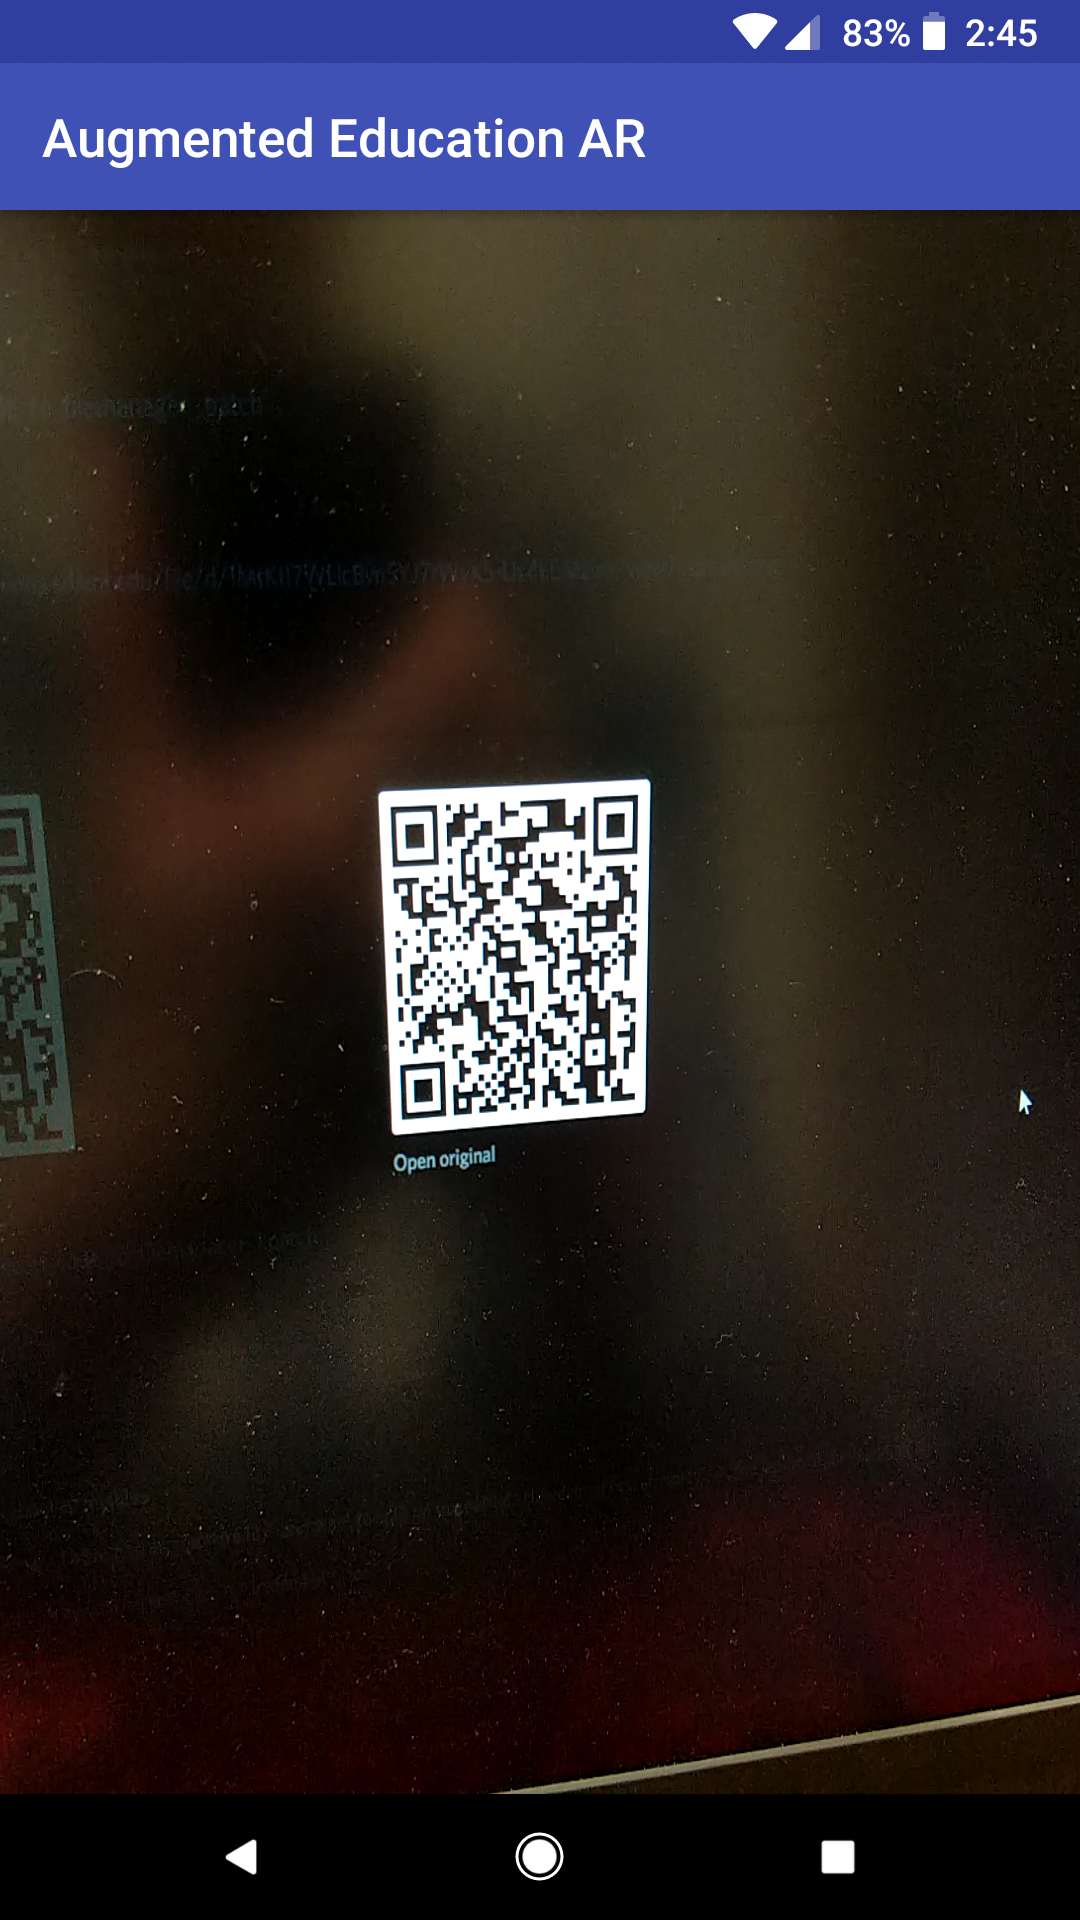
\includegraphics[width=0.5\textwidth]{Mobile/Mobile_QRScanning}
            \centering
            \caption{Mobile App - QR Code Reader}
            \label{fig:mobileQRScanning}
        \end{figure}

        \begin{figure}[H]
            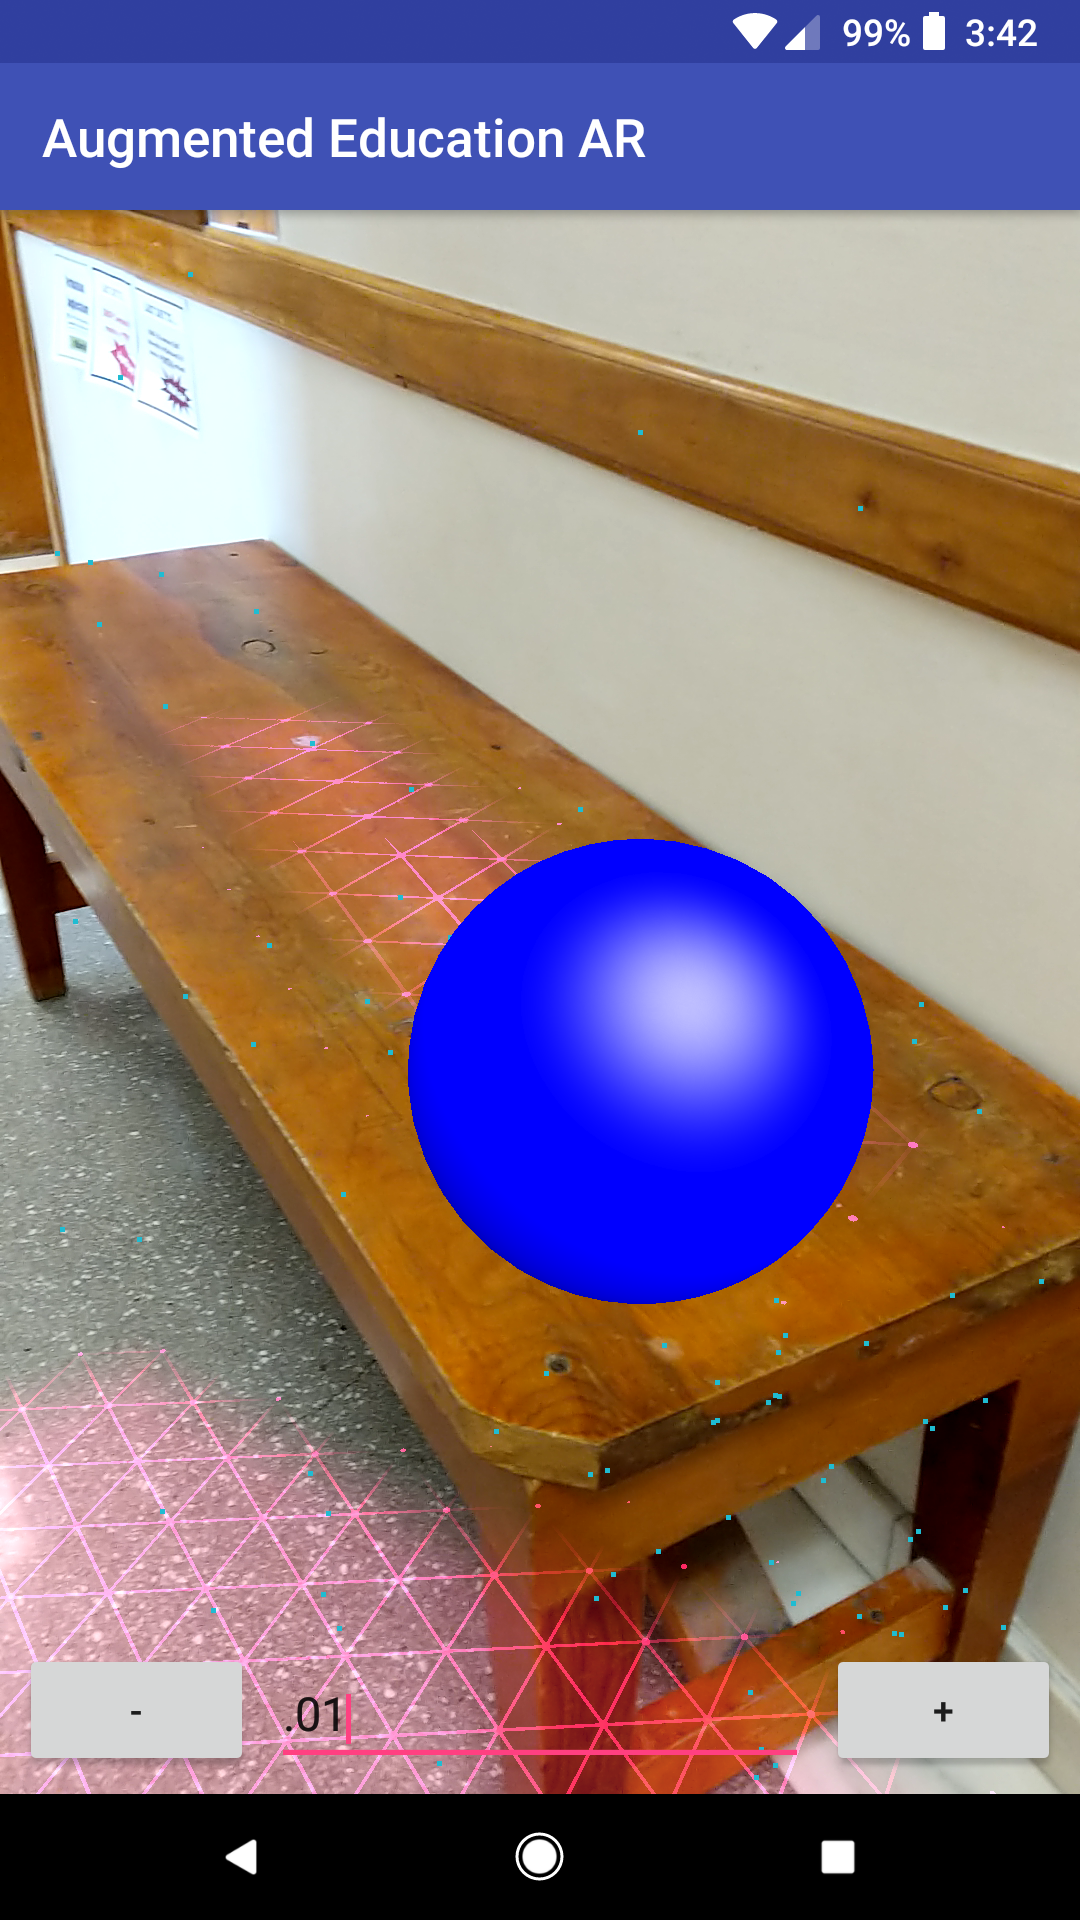
\includegraphics[width=0.5\textwidth]{Mobile/Mobile_BlueSphere}
            \centering
            \caption{Mobile App - AR Viewer}
            \label{fig:mobileModelViewer}
        \end{figure}

        \subsubsection{Activity Flow}

            When the user starts the app, the first screen is the \texttt{MainActivity}.  The main activity is where the user can enter their username and password, or continue offline.  If the user enters credentials, they are verified with the website, and an authentication token is passed to the next activity.  No matter which option the user chooses, the next activity is the \texttt{HomeActivity}.

            The \texttt{HomeActivity} displays a list of models for the user to choose from.  A series of models are included in the assets in the phone.  So whenever the user installs the app, a set of models always come with it.  Other models are populated by the website, or by QR codes.  When the activity starts, a request is sent to the website to get a list of models for that user.  Those models are added to the phone's database, so the files can be tracked.  A button for QR code scanning is also present on the view.  If the user taps that button, the QR code activity is started, and a QR code is read.  The value of the QR code is returned to the device, where the value is added to the database.  The user can then select a model from the list to start the AR Viewer.  If the model selected by the user is not downloaded on the phone, a request is made to the website for a file download.  A spinning progress bar is displayed by the QR button to show that there is activity.

            When the AR Viewer is started, the model selected is parsed and loaded.  If the file selected is large, it may take some time to move to the new activity.  When the user is done looking at the model, the back button can be pressed to return to the \texttt{HomeActivity}.
            
            During any of the activities, errors may occur.  When this happens, a toast is displayed on the screen.  A toast is a small, temporary box that appears on the lower section of the screen.  The duration for the toasts is typically set to short. 

            The activity flow for the mobile app can be seen in figure \ref{fig:mobileActivityFlow}

            \begin{figure}[H]
                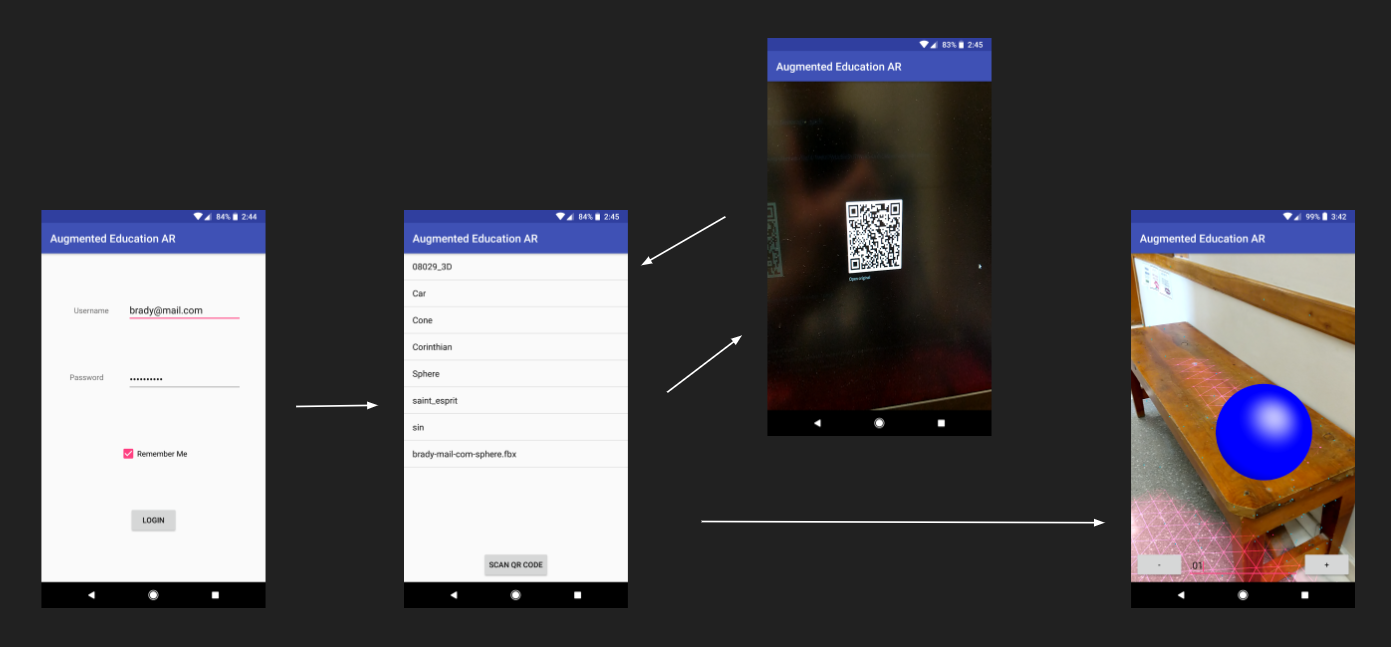
\includegraphics[width=\textwidth]{Mobile/Mobile_ActivityFlow}
                \centering
                \caption{Mobile App - Activity Flow}
                \label{fig:mobileActivityFlow}
            \end{figure}

